\documentclass[8pt,aspectratio=169]{beamer}
\usepackage[ruled,vlined]{algorithm2e}
\usepackage{amsmath}
\usepackage{amssymb}
\usepackage{amsfonts}
\usepackage{amsthm}
\usepackage{appendixnumberbeamer}
\usepackage[backend=biber, giveninits]{biblatex}
\usepackage{booktabs}
\usepackage{bm}
\usepackage{caption} 
\captionsetup[table]{skip=5pt}
\usepackage[scale=2]{ccicons}
\usepackage{color}
\usepackage{derivative}
\usepackage[inline,shortlabels]{enumitem}
\usepackage{epsfig}
\usepackage{expl3}
\usepackage{graphicx}
\usepackage{hyperref}
\usepackage{makecell}
\usepackage{mathtools}
\usepackage{multicol}
\usepackage{multirow}
\usepackage{placeins}
\usepackage{siunitx}
\usepackage{svg}
\usepackage{times}
\usepackage{xcolor}
\usepackage{xspace}
\usepackage{xparse}

%%%%%%%%% content delimiters
\NewDocumentCommand\secref{m}{Section~{\ref{#1}}}
\NewDocumentCommand\figref{m}{Figure~{\ref{#1}}}
\NewDocumentCommand\tabref{m}{Table~{\ref{#1}}}
\NewDocumentCommand\secsref{m}{Sections~{\ref{#1}}}
\NewDocumentCommand\figsref{m}{Figures~{\ref{#1}}}
\NewDocumentCommand\tabsref{m}{Tables~{\ref{#1}}}
\NewDocumentCommand\algref{m}{Algorithm~{\ref{#1}}}

%%%%%%%%% abbreviations
\makeatletter
\DeclareRobustCommand\onedot{\futurelet\@let@token\@onedot}
\def\@onedot{\ifx\@let@token.\else.\null\fi\xspace}
\def\eg{\emph{e.g}\onedot} \def\Eg{\emph{E.g}\onedot}
\def\ie{\emph{i.e}\onedot} \def\Ie{\emph{I.e}\onedot}
\def\cf{\emph{c.f}\onedot} \def\Cf{\emph{C.f}\onedot}
\def\etc{\emph{etc}\onedot} \def\vs{\emph{vs}\onedot}
\def\wrt{w.r.t\onedot} \def\dof{d.o.f\onedot}
\def\etal{\emph{et al}\onedot}
\makeatother

%%%%%%%%%% colors
\definecolor{mycolor1}{rgb}{0,0,0}%
\definecolor{mycolor2}{rgb}{1,0,1}%
\definecolor{mycolor3}{rgb}{0,1,1}%
\definecolor{mycolor4}{rgb}{0,0,1}%
\definecolor{mycolor5}{rgb}{0,1,0}%
\definecolor{betteryellow}{rgb}{1,0.8824,0.0980}
\definecolor{lavender}{rgb}{0.902,0.7451,1.0}
\definecolor{olive}{rgb}{0.5020,0.5020,0} 
\definecolor{orange}{rgb}{1,0.5,0} 
\definecolor{bettergreen}{rgb}{0,0.6,0.3}

\definecolor{blue}{HTML}{4069B0}
\definecolor{lightorange}{HTML}{FF8F00}
\definecolor{orange}{HTML}{E45611}
\definecolor{darkorange}{HTML}{B85325}
\definecolor{lightgreen}{HTML}{34DC5B}
\definecolor{green}{HTML}{28A745}
\definecolor{lightgray}{HTML}{656972}
\definecolor{gray}{HTML}{53585F}
\definecolor{darkgray}{HTML}{333333}
\definecolor{red}{HTML}{D61901}
\definecolor{magenta}{HTML}{CC00CC}
\definecolor{cyan}{HTML}{00FFFF}

\def\firstpl#1{\textcolor{bettergreen}{\textbf{#1}}}
\def\secondpl#1{\textcolor{lightorange}{\textbf{#1}}}
\def\stateofart#1{\textbf{#1}}
\def\red#1{\textcolor{red}{\textbf{#1}}}

\newcommand{\mycbox}[1]{\tikz{\path[draw=#1,fill=#1] (0,0) rectangle (5pt,5pt);}}
\DeclareMathOperator{\rank}{rank}%
\DeclareMathOperator{\vect}{vec}%
\DeclareMathOperator{\atantwo}{atan2}%
\DeclareMathOperator*{\argmin}{argmin}%
\DeclareMathOperator*{\argmax}{argmax}%

\DeclarePairedDelimiter{\abs}{\lvert}{\rvert}
\DeclarePairedDelimiter{\norm}{\lVert}{\rVert}
\DeclarePairedDelimiter{\innerproduct}{\langle}{\rangle}

\DeclarePairedDelimiter{\parenfences}{(}{)}
\DeclarePairedDelimiter{\brackets}{[}{]}
\DeclarePairedDelimiter{\coord}{(}{)}
\DeclarePairedDelimiterX{\sksym}[1]{[}{]_{\times}}{#1}

% just to make sure it exists
\providecommand\given{}
% can be useful to refer to this outside \Set
\newcommand\SetSymbol[1][]{%
\nonscript\:#1\vert
\allowbreak
\nonscript\:
\mathopen{}}

\DeclarePairedDelimiterX\set[1]\{\}{%
\,\renewcommand\given{\SetSymbol[\delimsize]}
#1\,
}

\NewDocumentCommand\Zz{}{\mathbb{Z}} % Integsers
%\NewDocumentCommand\Re{}{\mathbb{R}} % Reals
\NewDocumentCommand\Rp{}{\mathbb{RP}} % Real-Projective Space

\NewDocumentCommand\Lgn{}{\mathcal{L}} % Lagrangian

\NewDocumentCommand{\vertbar}{}{\rule[-1ex]{0.5pt}{2.5ex}}
\NewDocumentCommand{\horzbar}{}{\rule[.5ex]{2.5ex}{0.5pt}}

\NewDocumentCommand\sqnorm{m}{\norm{#1}^2} % inverse transpose
\NewDocumentCommand\sqltwonorm{m}{\norm{#1}_2^2} % inverse transpose
\NewDocumentCommand\inv{}{\mathsf{-1}} % inverse transpose
\NewDocumentCommand\T{}{\top} % transpose
\NewDocumentCommand\invT{}{-\top} % inverse transpose
\NewDocumentCommand\diag{}{\operatorname{diag}\parenfences}

\NewDocumentCommand\dist{O{}}{d_{\text{#1}}\parenfences}
\NewDocumentCommand\sqdist{O{}}{d_{\text{#1}}^2\parenfences}
\NewDocumentCommand\gaussian{}{\mathcal{N}\parenfences}

\DeclareMathOperator{\EE}{\mathbb{E}}

\newcommand*\rot{\rotatebox{90}}

\NewDocumentCommand\cspond{mm}{#1\leftrightarrow#2}

\NewDocumentCommand\removebslash{m}{%
  {\catcode92=9 \endlinechar-1 \scantokens{#1}}%
}

\NewDocumentCommand\vecbold{m}{\bm{#1}}

\ExplSyntaxOn

\NewDocumentCommand\definevecbold{m}
{
  \clist_map_inline:nn { #1 }
  {
    \cs_new_protected:cpn { vb##1 } { \vecbold{##1} }
  }
}

\NewDocumentCommand{\defineset}{m}
{
  \clist_map_inline:nn { #1 }
  {
    \cs_new_protected:cpn { s##1 } { \mathcal{##1} }
  }
}

\clist_new:N \vectr_clist
\NewDocumentCommand{\vectr}{O{\\}mO{b}}{
  \clist_set:Nn \vectr_clist {#2} % Set the list
  \begin{#3matrix}
  \clist_use:Nn \vectr_clist {#1} % show it with separator from #1 (\\)
  \end{#3matrix}
}

\NewDocumentCommand{\rvec}{mO{b}}{\vectr[&]{#1}[#2]}
\NewDocumentCommand{\cvec}{mO{b}}{\vectr{#1}[#2]}

\NewDocumentCommand{\rmat}{mO{b}}{
  \clist_set:Nn \l_rmat_clist {#1} % Set the list
  \begin{#2matrix}
    \horzbar &
    \clist_use:Nn \l_rmat_clist {& \horzbar \\ \horzbar &}  % show it with separator from #1 (\\)
    & \horzbar
  \end{#2matrix}
}

\NewDocumentCommand{\cmat}{mO{b}}{
  \clist_set:Nn \l_cmat_clist {#1} % Set the list
  \begin{#2matrix}
    & \clist_map_inline:Nn \l_cmat_clist { \vertbar & } \\
    & \clist_use:Nn \l_cmat_clist {& } \\ % Set the list
    & \clist_map_inline:Nn \l_cmat_clist { \vertbar & } \\
  \end{#2matrix}
}

\ExplSyntaxOff

\definevecbold{A,B,C,D,E,F,H,I,J,K,M,P,Q,R,T,U,V,W,X,Y,Z,a,b,c,d,e,f,h,l,m,n,o,p,r,t,u,v,x,y,z}
\defineset{A,B,C,D,E,F,G,H,I,J,K,L,M,N,O,P,Q,R,S,T,U,V,W,X,Y,Z}

\NewDocumentCommand\linf{}{\vbl_\infty}
\NewDocumentCommand\vbSigma{}{\vecbold{\Sigma}}
\NewDocumentCommand\vbphi{}{\vecbold{\phi}}
\NewDocumentCommand\vbzero{}{\vecbold{0}}
\NewDocumentCommand\vbdelta{}{\vecbold{\delta}}
\NewDocumentCommand\vbepsilon{}{\vecbold{\epsilon}}
\NewDocumentCommand\vbmu{}{\vecbold{\mu}}

\def\mKRt{\ensuremath{\mK \begin{bmatrix} \mR & \vt \end{bmatrix}}}

\newcommand*\Let[2]{\State #1 $\gets$ #2}

\def\mupinvof#1{{{#1}^{-\lambda}}}

\newcommand{\eps}{\varepsilon}
\providecommand{\homogvec}[1]{\binom{n}{1}}
\providecommand{\dotprod}[2]{\left\langle #1, #2 \right\rangle}

\newenvironment{smallpmatrix}{\left(\begin{smallmatrix}}{\end{smallmatrix}\right)}


\newcommand{\cmark}{\ding{51}}%
\newcommand{\xmark}{\ding{55}}%
\setlength\aboverulesep{0pt}
\setlength\belowrulesep{0pt}

\newtheorem*{remark}{Remark}
\newtheorem*{desiderata}{Desiderata}
\newtheorem*{result}{Result}



\NewDocumentCommand\pinhole{}{\pi\parenfences}
\newcommand{\RANSAC}{RANSAC\xspace}
\setbeamertemplate{frametitle} 
{
  \begin{centering}
    \smallskip 
    \insertframetitle\par 
    \smallskip
  \end{centering}} 

\setbeamertemplate{itemize item}{$\bullet$} 
\setbeamertemplate{navigation symbols}{} 
\setbeamertemplate{footline}[text line]{% 
  \hfill\strut{% 
    \scriptsize\sf\color{black!60}% 
    \quad\insertframenumber 
  }% 
  \hfill 
} 

\setbeamerfont{title}{size=\Huge}
\setbeamerfont{frametitle}{size=\LARGE}

% Define some colors: 
\definecolor{DarkFern}{HTML}{407428} 
\definecolor{DarkCharcoal}{HTML}{4D4944} 
\colorlet{Fern}{DarkFern!85!white} 
\colorlet{Charcoal}{DarkCharcoal!85!white} 
\colorlet{LightCharcoal}{Charcoal!50!white} 
\colorlet{AlertColor}{orange!80!black} 
\colorlet{DarkRed}{red!70!black} 
\colorlet{DarkBlue}{blue!70!black} 
\colorlet{DarkGreen}{green!70!black} 
\definecolor{purple(munsell)}{rgb}{0.62, 0.0, 0.77}
% Use the colors: 
\setbeamercolor{title}{fg=purple} 
\setbeamercolor{frametitle}{fg=purple} 
\setbeamercolor{normal text}{fg=black} 
\setbeamercolor{block title}{fg=purple,bg=white} 
\setbeamercolor{block body}{fg=black,bg=white} 
\setbeamercolor{alerted text}{fg=AlertColor} 
\setbeamercolor{itemize item}{fg=Charcoal}

\let\oldblock\block
\let\endoldblock\endblock

% change block by adding smallskip
\renewenvironment{block}[1]
{\begin{oldblock}{#1}
    \smallskip
  }
  { 
  \end{oldblock}
}

\addbibresource{notes.bib}

\logo{
\includegraphics{img/logo-en}}

\setcounter{MaxMatrixCols}{20}

\title{Covariance Propagation}
\subtitle{Propogation through an unconstrained solver}
\date{\today}
\author{James Pritts}
\institute{Ukrainian Catholic University}
\titlegraphic{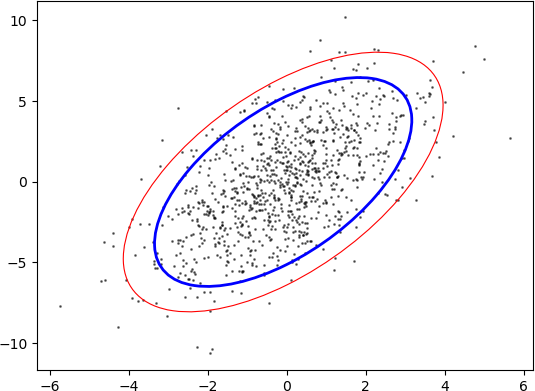
\includegraphics[height=2.5cm]{img/covariance.png}}

\begin{document} 

\maketitle

\begin{frame}{Table of contents}
  \setbeamertemplate{section in toc}[sections numbered]
  \tableofcontents%[hideallsubsections]
\end{frame}

\section[Intro]{Introduction}

\begin{frame}[fragile]{Measurement Errors}
  Can we improve vision algorithms by modeling inexact measurements?

  \begin{itemize}
  \item Errors accumulate during measurement. 
  \item Vision algorithms assume measurements are exact.
  \item Photogrammetry typically incorporates error analysis.
  \end{itemize}
\end{frame}

\begin{frame}[fragile]{Random Errors}
  \begin{definition}{Random errors} in experimental measurements are caused by unknown and unpredictable changes in the experiment.
  \end{definition}

  \begin{itemize}
    \item Errors are introduced by the feature extractor or the environmental conditions.
    \item An example of a source of random error is CCD noise.
  \end{itemize}
\end{frame}

\begin{frame}[fragile]{Modeling Random Errors}
  We assume that our feature extractors do not have systematic error,
  or that they are unbiased estimators.
  
  \begin{itemize}
  \item Measurements are modeled as random variables.
  \item The measurement is the sum of many unobserved random factors.
  \item The Central Limit Theorem is used to justify the
    representation of measurements as Gaussian random vectors.
  \end{itemize}
\end{frame}

%\section{Titleformats}

\begin{frame}[fragile]{Linear Transformation of a Distribution}
  \begin{theorem}
    Suppose $\vX \sim p_{\vX}(\vx)$ and $\ma{J}$ is an an invertible matrix. Then the 
    density of $\vY = \ma{J}\vX$ is 
    \[p_{\vY}(\vy) = \frac{p_{\vX} (\inv{\ma{J}} \vy)}{| \det \ma{J} |} \]
  \end{theorem}
\end{frame}

\begin{frame}[fragile]{Linear Transformation of a Gaussian is Gaussian}
  \begin{theorem}
    Suppose $\vX \sim \mathcal{N}(\mu_{\vX},\Sigma_{\vX})$ and
    $\ma{J}$ is an an invertible matrix. Then the density of $\vY =
    \ma{J}\vX$ is
    \begin{align*}
      p_{\vY}(\vy) &= \frac{p_{\vX}(\inv{\ma{J}} \vy)}{| \det \ma{J} |}  \\
      &= \mathcal{N}(\ma{J}\vX,\ma{J}\Sigma_{\vX}\ma{J}^{\T})  \\
      &= \mathcal{N}(\vY,\Sigma_{\vY})  \\
    \end{align*}
  \end{theorem}
\end{frame}

\begin{frame}[fragile]{Explicit Function}
  Suppose $\vy = \vy(\vx)$ and let $\vx = \mu_{\vx}+\Delta\vx$. Linearize $\vy$ about $\mu_{\vx}$,
  \[
  \vy(\mu_{\vx}+\Delta\vx)=\vy(\mu_{\vx})+\ma{J}_{\vy}(\mu_{\vx})\Delta \vx + \mathcal{O}(\|\Delta\vx\|^2)
  \]

  Start with the definition of the covariance for the output $\vy$
  \begin{align*}
    \Sigma_{\vy} &= \mathbb{E}\left[(\vy-\mu_{\vy})(\vy-\mu_{\vy})^{T}\right] \\
    &= \mathbb{E}\left[\left(\vy(\mu_{\vx}+\Delta\vx)-\mu_{\vy}\right)\left(\vy(\mu_{\vx}+\Delta\vx)-\mu_{\vy}\right)^{T}\right] 
  \end{align*}

  Assume $\mu_{\vy} \approx \vy(\mu_{\vx})$ and $\vy(\mu_{\vx}+\Delta\vx) \approx \vy(\mu_{\vx})+\nabla \vy(\mu_{\vx})\Delta \vx$, then 
  \begin{align*}
    \Sigma_{\vy} & \approx \mathbb{E}\left[\left(\vy(\mu_{\vx}+\Delta\vx)-\vy(\mu_{\vx})\right)\left(\vy(\mu_{\vx}+\Delta\vx)-\vy(\mu_{\vx})\right)^{T}\right] \\
    & \approx \mathbb{E}\left[\ma{J}_{\vy}(\mu_{\vx})\Delta\vx\Delta\vx^{\T}\ma{J}_{\vy}(\mu_{\vx})^{\T}\right] \\
    & \approx \ma{J}_{\vy}(\mu_{\vx})\Sigma_{\vx}\ma{J}_{\vy}(\mu_{\vx})^{\T}
  \end{align*}
  
  $\mu_{\vx}$ is unknown, but if $\Delta\vx$ is small
  \begin{equation}
    \Sigma_{\vy} \approx \ma{J}_{\vy}(\vx)\Sigma_{\vx}\ma{J}_{\vy}(\vx)^{\T}.
    \label{eq:cov_prop}
  \end{equation}
\end{frame}

\begin{frame}[fragile]{Regression}
  Given some measurements $\vx$ and a differentiable
  objective $\mathcal{J}$, solve for parameters $\vy^{*}$
  by
  \[ \vy^{*} = \argmin_{\vy} \mathcal{J}(\vx,\vy) \]

  Satisfying the constraint
  \[  \diffp*{\mathcal{J}(\vx,\vy)}{\vy}{(\vx[0],\vy^{*})} = 0. \]
  is a necessary condition for $\vy^{*}$ to be a local minimium for
  measurements \vx[0].

  \vspace{1em}

  Referring to (1), we require $\ma{J}_{\vy}(\vx)$ to propogate.
\end{frame}

\begin{frame}[fragile]{Implicit Function Theorem}
  \begin{theorem}
    Suppose $\vphi(\vx,\vy)$ is differentiable,
    $\vphi(\vx[0],\vy^{*})=\v0$ and $\left|
    \diffp*{\vphi}{\vy}{(\vx[0],\vy^{*})} \right| \neq 0$. Then there
    is a unique and differentiable function $\vy(\vx)$ in the
    neighborhood of $(\vx[0],\vy^{*})$ so that
    $\vphi(\vx,\vy(\vx))=\v0$.
  \end{theorem}
  \vspace{1em}
  The parametric form of $\vy(\vx)$ may be unknown.
\end{frame}


\begin{frame}[fragile]{Implicit Differentiation}
  Suppose there are sufficient conditions on \vphi \xspace to invoke the
  Implicit Function Theorem. Then we can derive the expression for
  $\ma{J}_{\vy}$.

  \vspace{1em}
  Impilcitly differentiate $\vphi$,
  \[
  \diff{\vphi}{\vx} = \diffp{\vphi}{\vx}+\diffp{\vphi}{\vy}\diff{\vy}{\vx} = \v0
  \]

  and solve for   $\diff{\vy}{\vx}$

  \[
  \diff{\vy}{\vx} = -\inv{\left( \diffp{\vphi}{\vy} \right)} \diffp{\vphi}{\vx}
  \]

  where 
  \begin{equation}
    \ma{J}_{\vy} = \diff{\vy}{\vx}.
  \end{equation}
\end{frame}

\begin{frame}[fragile]{Propogating through Unconstrainted Optimization}
  Let $\vphi(\vx,\vy) = \diffp{\mathcal{J}(\vx,\vy)}{\vy}$ and suppose
  $\diffp*{\mathcal{J}(\vx,\vy)}{\vy}{(\vx[0],\vy^{*})} =
  \v0$.

  \vspace{1em}

  Applying (2), we have

  \begin{equation}
    \ma{J}_{\vy} = \inv{\left(\diffp[2]{\mathcal{J}}{\vy}\right)}\diffp{\mathcal{J}}{\vy\vx}
  \end{equation}

  Let $\ma{H}_{\mathcal{J}}$ be the hessian of $\mathcal{J}$ w.r.t. \vy, and substitute

  \begin{equation}
    \ma{J}_{\vy} = \ma{H}_{\mathcal{J}} \diffp{\vphi}{\vx}
  \end{equation}
  
\end{frame}


%\begin{frame}[fragile]{Gauss-Newton Approximation to the Hessian}
%  Suppose $\mathcal{J}(\vx,\vy)=\|\ve(\vx,\vy)\|_2^2$.
%  \vspace{1em}y
%  Then
%  \[
%  \ma{H}_{\mathcal{J}} = 2\left(\ma{J}^{\T}_{\mathcal{J}}\ma{J}_{\mathcal{J}}+\sum_i e_i(\vx,\vy)^{\T} \right)
%  \]
%\end{frame}

\begin{frame}
  Then (1) can be applied to propogate the covariance

  \begin{equation}
    \Sigma_{\vy} \approx \ma{J}_{\vy}(\vx)\Sigma_{\vx}\ma{J}_{\vy}(\vx)^{\T}.
  \end{equation}
\end{frame}

\begin{frame}[fragile]{Seven-point Method}
  The fundamental matrix \mF\xspace is a rank-two matrix that relates
  pt. correspondences, denoted $\{\,\cspond{\vx[i]}{\vxp[i]}\,\}$, in
  stereo images.
  \medskip

  The epioplar line $\vl = \ma{F}\vx$ in the second image contains \vxp.
  \medskip

  This epipolar constraint $\vx^{\prime \T} \ma{F} \vx=0$ can be
  written as
  \[
    \label{eq:billinear_form}
    \vm^{\T}_i \operatorname{vec}(\ma{F}) = \vx[i] \otimes \vxp[i]  \operatorname{vec}(\ma{F}) = 0.
    \]

  $\ma{F}$ has 7 degrees of freedom, so 7 equations are needed.
  \medskip  

  Letting $\vf = \operatorname{vec}(\ma{F}^{\T})$ we have
  \[
  \ma{M}\vf = \v0
  \]
  where $\ma{M} \in \R[7 \times 9]$
\end{frame}

\begin{frame}[fragile]{Imposing Rank Two Constraint}
  Denote the null space basis vectors of $\ma{M}$ as $\vf_1$ and $\vf_2$.
  \medskip
  
  $\ma{F}$ is singular so,
  \[\det \inv{\operatorname{vec}_{3\times3}} (\vf_1+\alpha_i \vf_2) = 0\]

  One or three real solutions for $\alpha$ are used to construct $\ma{F}_i$
  \begin{equation}
    \label{eq:estimateF}
    \ma{F}_i = \inv{\operatorname{vec}_{3\times3}} (\vf_1+\alpha_i \vf_2)^{\T}.
  \end{equation}

  Let $\ma{F} \in \{ \ma{F}_i \}$ be a solution.
  \medskip
  Given nonzero $\lambda$, $\lambda \ma{F}^{*}_i$ is also a solution.
  \medskip
  
  Restrict solutions to lie on the hypersphere
  \[
  \ma{F}^{*} = \frac{\ma{F}}{\| \ma{F}^{*} \|}
  \]
\end{frame}

\begin{frame}[fragile]{Covariance Propagation}
  Consider the constraint equations as residuals, namely
  \[
  \mathcal{J}(\vx,\vf)= \| \ma{M}\vf \|^2 = \|\vepsilon \|^2 = \sum_i \vepsilon_i^2  = \sum_i \| \vx[i]^{\prime \T} \ma{F} \vx[i] \|^2
  \]
  
  Let $\ma{F}^{*}$ be computed for measurements \vx[0] by the seven-point method.
  \bigskip

  $\mathcal{J}(\vx[0],\vf^{*})$ is 0, so  $\diffp*{\mathcal{J}(\vx,\vf)}{\vf}{(\vx[0],\vf^{*})} = \v0$.
\end{frame}

\begin{frame}
  $\vf^{*}$ is not a minimial parameterization.
  \bigskip

  We must account for the rank two constaint and scale ambiguity.
  \bigskip
  
  Let $\alpha,\beta \in \R,$ amd $g_2 \in \R[3]$ and $g_3 \in \R[2]$, and $g_1 = \alpha g_2 + \beta \colvec{2}{g_3}{f_{33}}$

  Then parameter vector $\theta = (\alpha,\beta,g_2,g_3)$
  \[
  \vf(\theta) = \colvec{4}{g_1}{g_2}{g_3}{f_{33}}
  \]

  and the objective becomes $\mathcal{J}(\vx,\theta)$
\end{frame}

\begin{frame}
  \begin{equation}
    \ma{J}_{\theta} = \inv{\left(\diffp[2]{\mathcal{J}}{\theta}\right)}\diffp{\mathcal{J}}{\theta \vx}
  \end{equation}
  \bigskip
  where $\ma{J}_{\theta} \in \R[7 \times 28]$ so that $\Sigma_{\theta} = \ma{J}_{\theta}\Sigma_{\vx}\ma{J}^{\T}_{\theta} $

  \bigskip
  and

  \bigskip
  $\ma{J}_{\vf} = \diff{\vf}{\theta}$ so that  $\Sigma_f = \ma{J}_{\vf} \Sigma_{\theta} \ma{J}^{\T}_{\vf}$.


\end{frame}

\end{document}
